\documentclass[12pt]{article}
\usepackage[utf8]{inputenc}
\usepackage[left=2cm,right=2cm,top=2cm,bottom=2cm]{geometry}
\usepackage{graphicx}
\usepackage[small]{caption}
\usepackage{subcaption}
\usepackage[spanish]{babel}
\usepackage{url}
\setlength{\parskip}{\baselineskip}
\graphicspath{ {images/} }


\usepackage{hyperref}
\hypersetup{
	colorlinks=true,
	linkcolor=blue,     
	urlcolor=blue,
	citecolor=blue,
}


\begin{document}


	\thispagestyle{empty}

	\begin{center}
		{\Large \bf Distribuciones de probabilidad geométrica, binomial y binomial negativa.}\\
		Gabriela S\'anchez Y.\\
		5064
	\end{center}
 
	En el presente trabajo se analiza el tipo de distribuciones que pueden están presentes en el texto del libro \textit{``Anne of Green Gables''} \cite{anne} que puede obtenerse de manera gratuita en el sitio de \href{http://www.gutenberg.org/}{Project Gutenberg}.

	\section{Introducción}
	
	El procesamiento del texto se realiza con la ayuda del lenguaje de programación \textsc{R} versión 4.0.2 \cite{r}, haciendo uso de distintas librerías:: \texttt{gutenbergr} que permite acceder al texto plano del libro y, \texttt{tidytext} y \texttt{dplyr} que permiten la descomposición del texto. 
	
	En el preprocesamiento se eliminan las líneas vacías, el índice y los guiones bajos cuando hay palabras con guiones bajos alrededor para indicar énfasis \cite{mpa_alberto}. Para tener un punto de comparación sobre lo que es propio del autor en la escritura de un texto se elige un cuento cuya fecha de publicación no se aleja mucho de la del libro base. En este caso se utiliza el libro \textit{Peter Pan} \cite{peterpan} que se descarga del mismo sitio \cite{pg}.
	
	El procedimiento realizado para el análisis puede encontrarse en el código \texttt{t3.R} \cite{mpa_gaby}.

	\section{Distribuciones en el texto}
	
	En esta fase se descompone el texto en oraciones, es decir, se parte después de cada punto. La comparación se realiza a partir de la medición de la cantidad de palabras, y comas que hay en las oraciones de cada texto. Además se analiza la longitud de las palabras usadas.
	
	En la figura \ref{anne_peter} se puede observar una síntesis de cómo están distribuidos estos elementos en las oraciones de cada texto. En general, tienen un comportamiento similar. Se podría decir que la distribución de la cantidad de palabras por oración en ambos textos (figura \ref{ppo_anne} y \ref{ppo_peter}) y la distribución de la cantidad de comas por oración (figura \ref{cpo_anne} y \ref{cpo_peter}) es muy similar a una distribución geométrica. 
	
	\begin{figure}
		\begin{subfigure}{.5\textwidth}
			\centering
			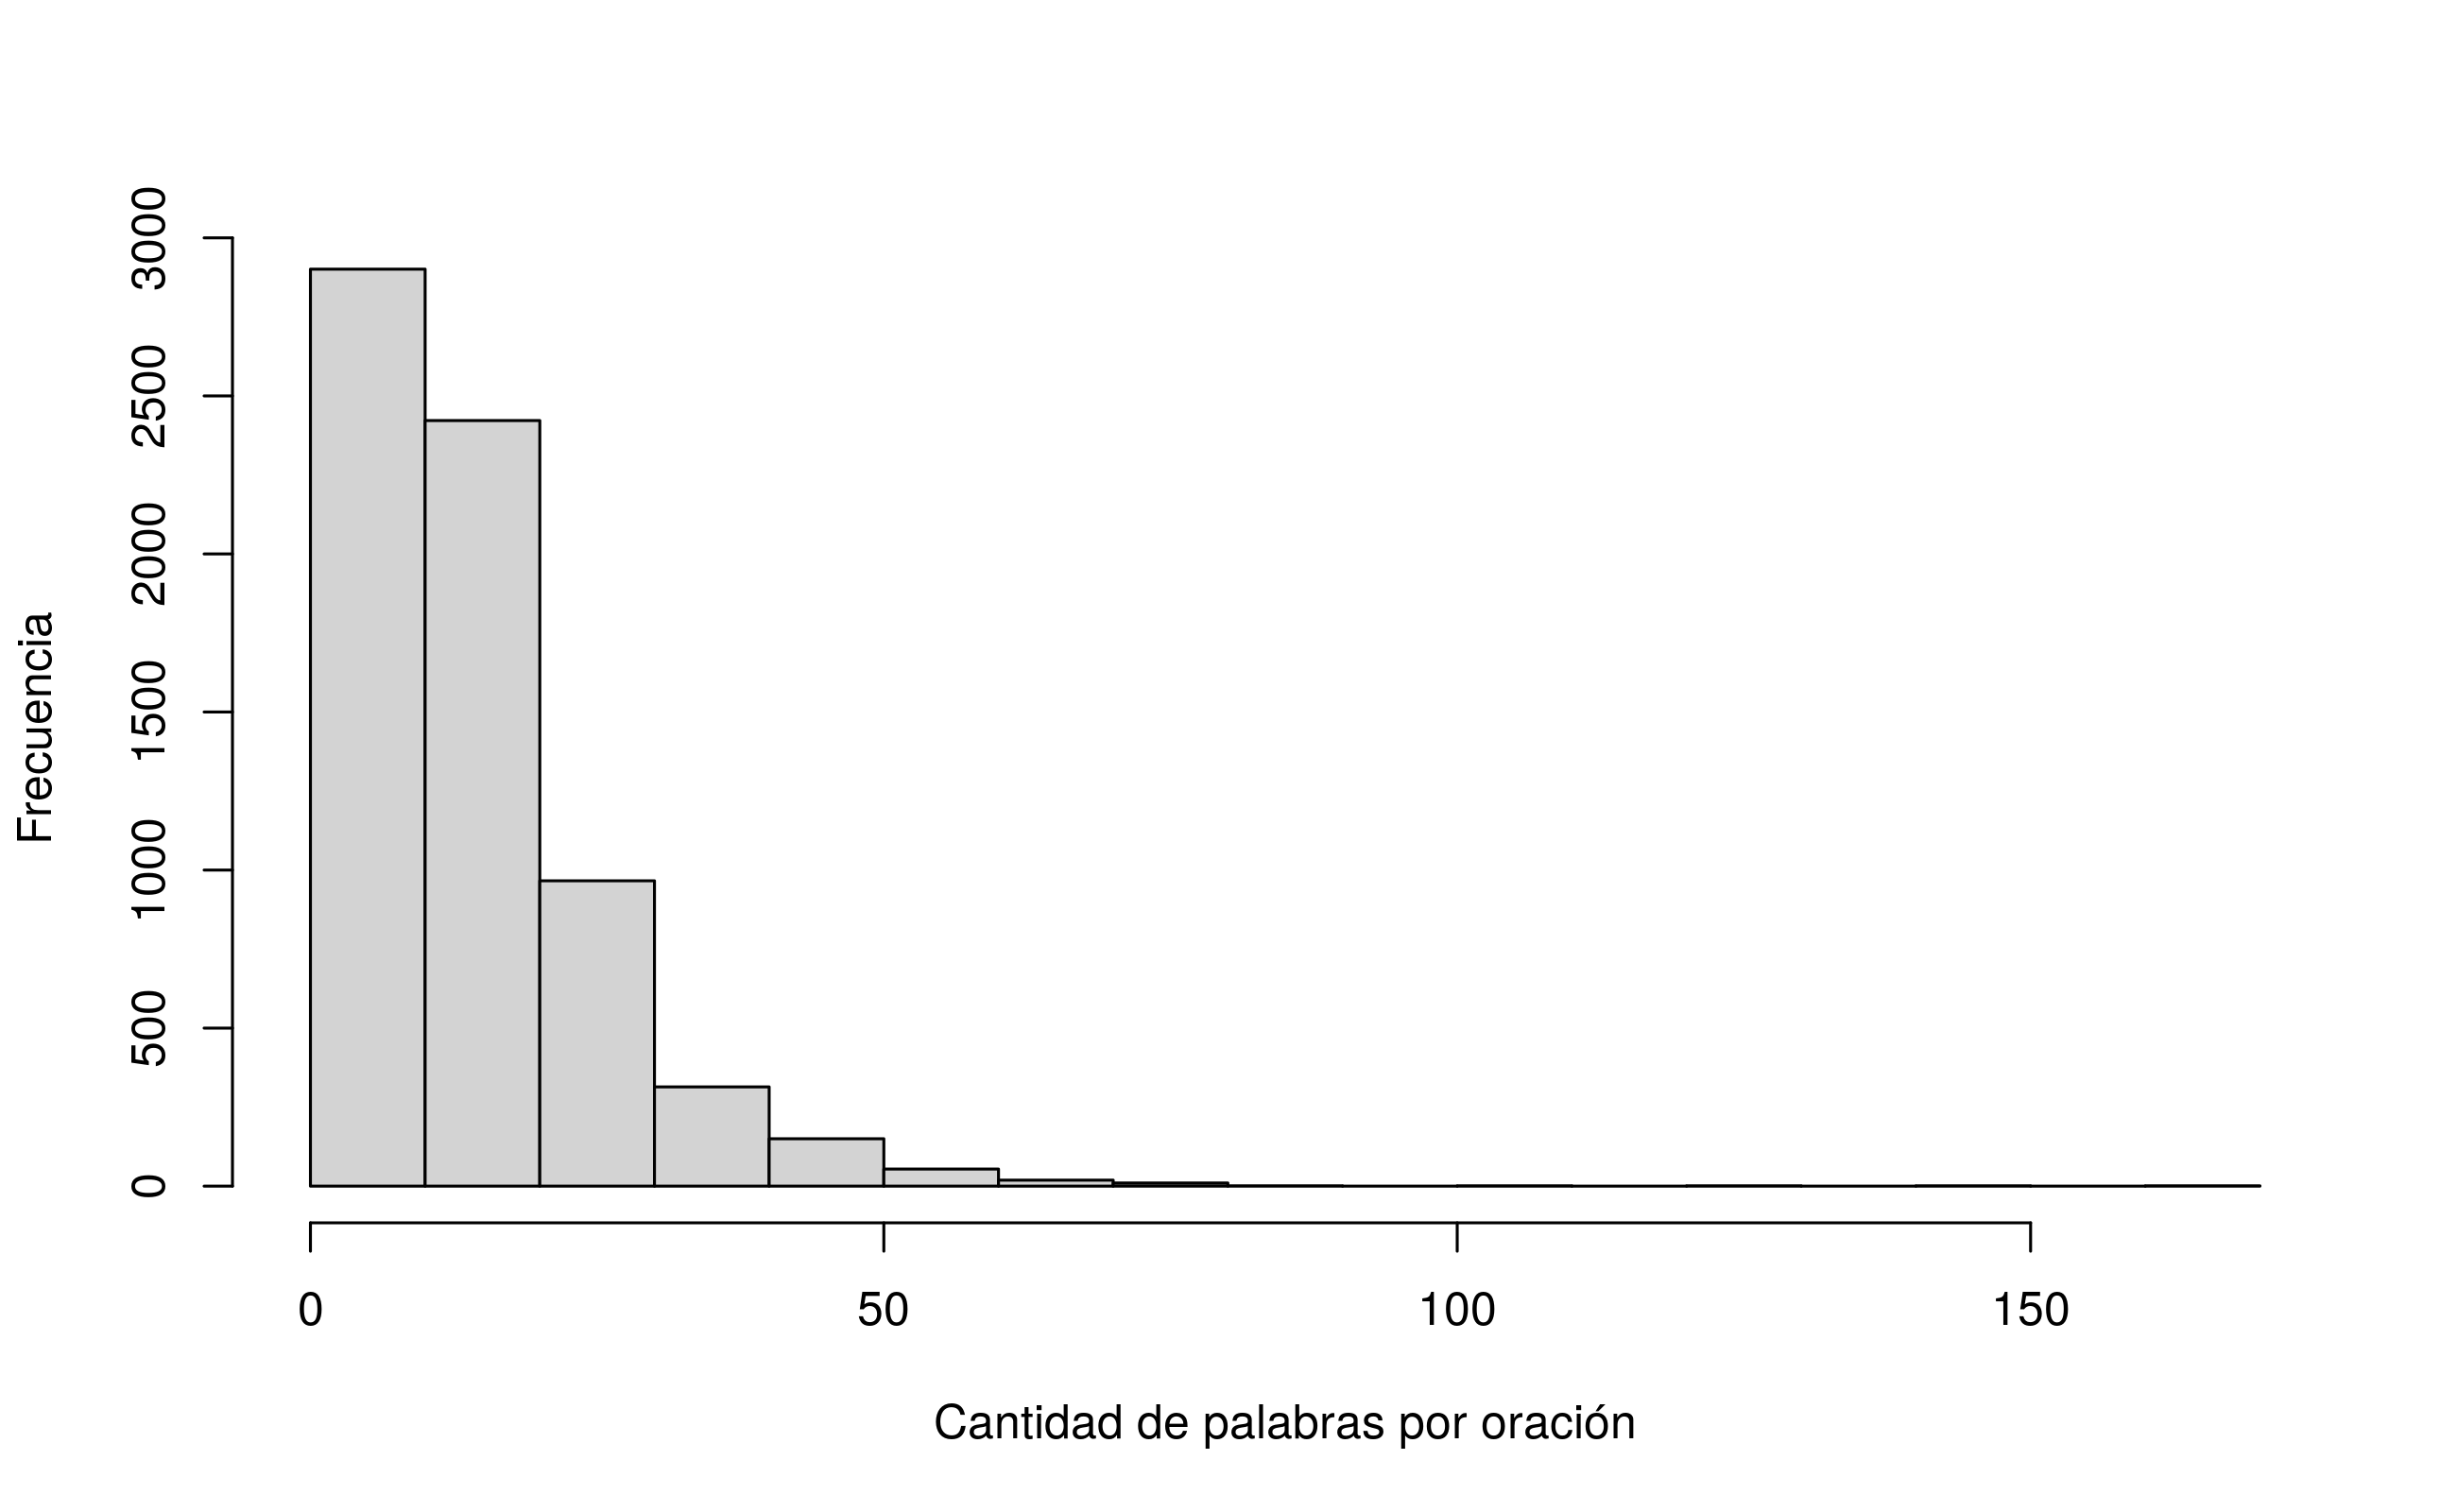
\includegraphics[scale=0.4]{hist_ppo_anne.png}
			\caption{Palabras por oración en \em Anne of Green Gables}
			\label{ppo_anne}
		\end{subfigure}
		\begin{subfigure}{0.5\textwidth}
			\centering
			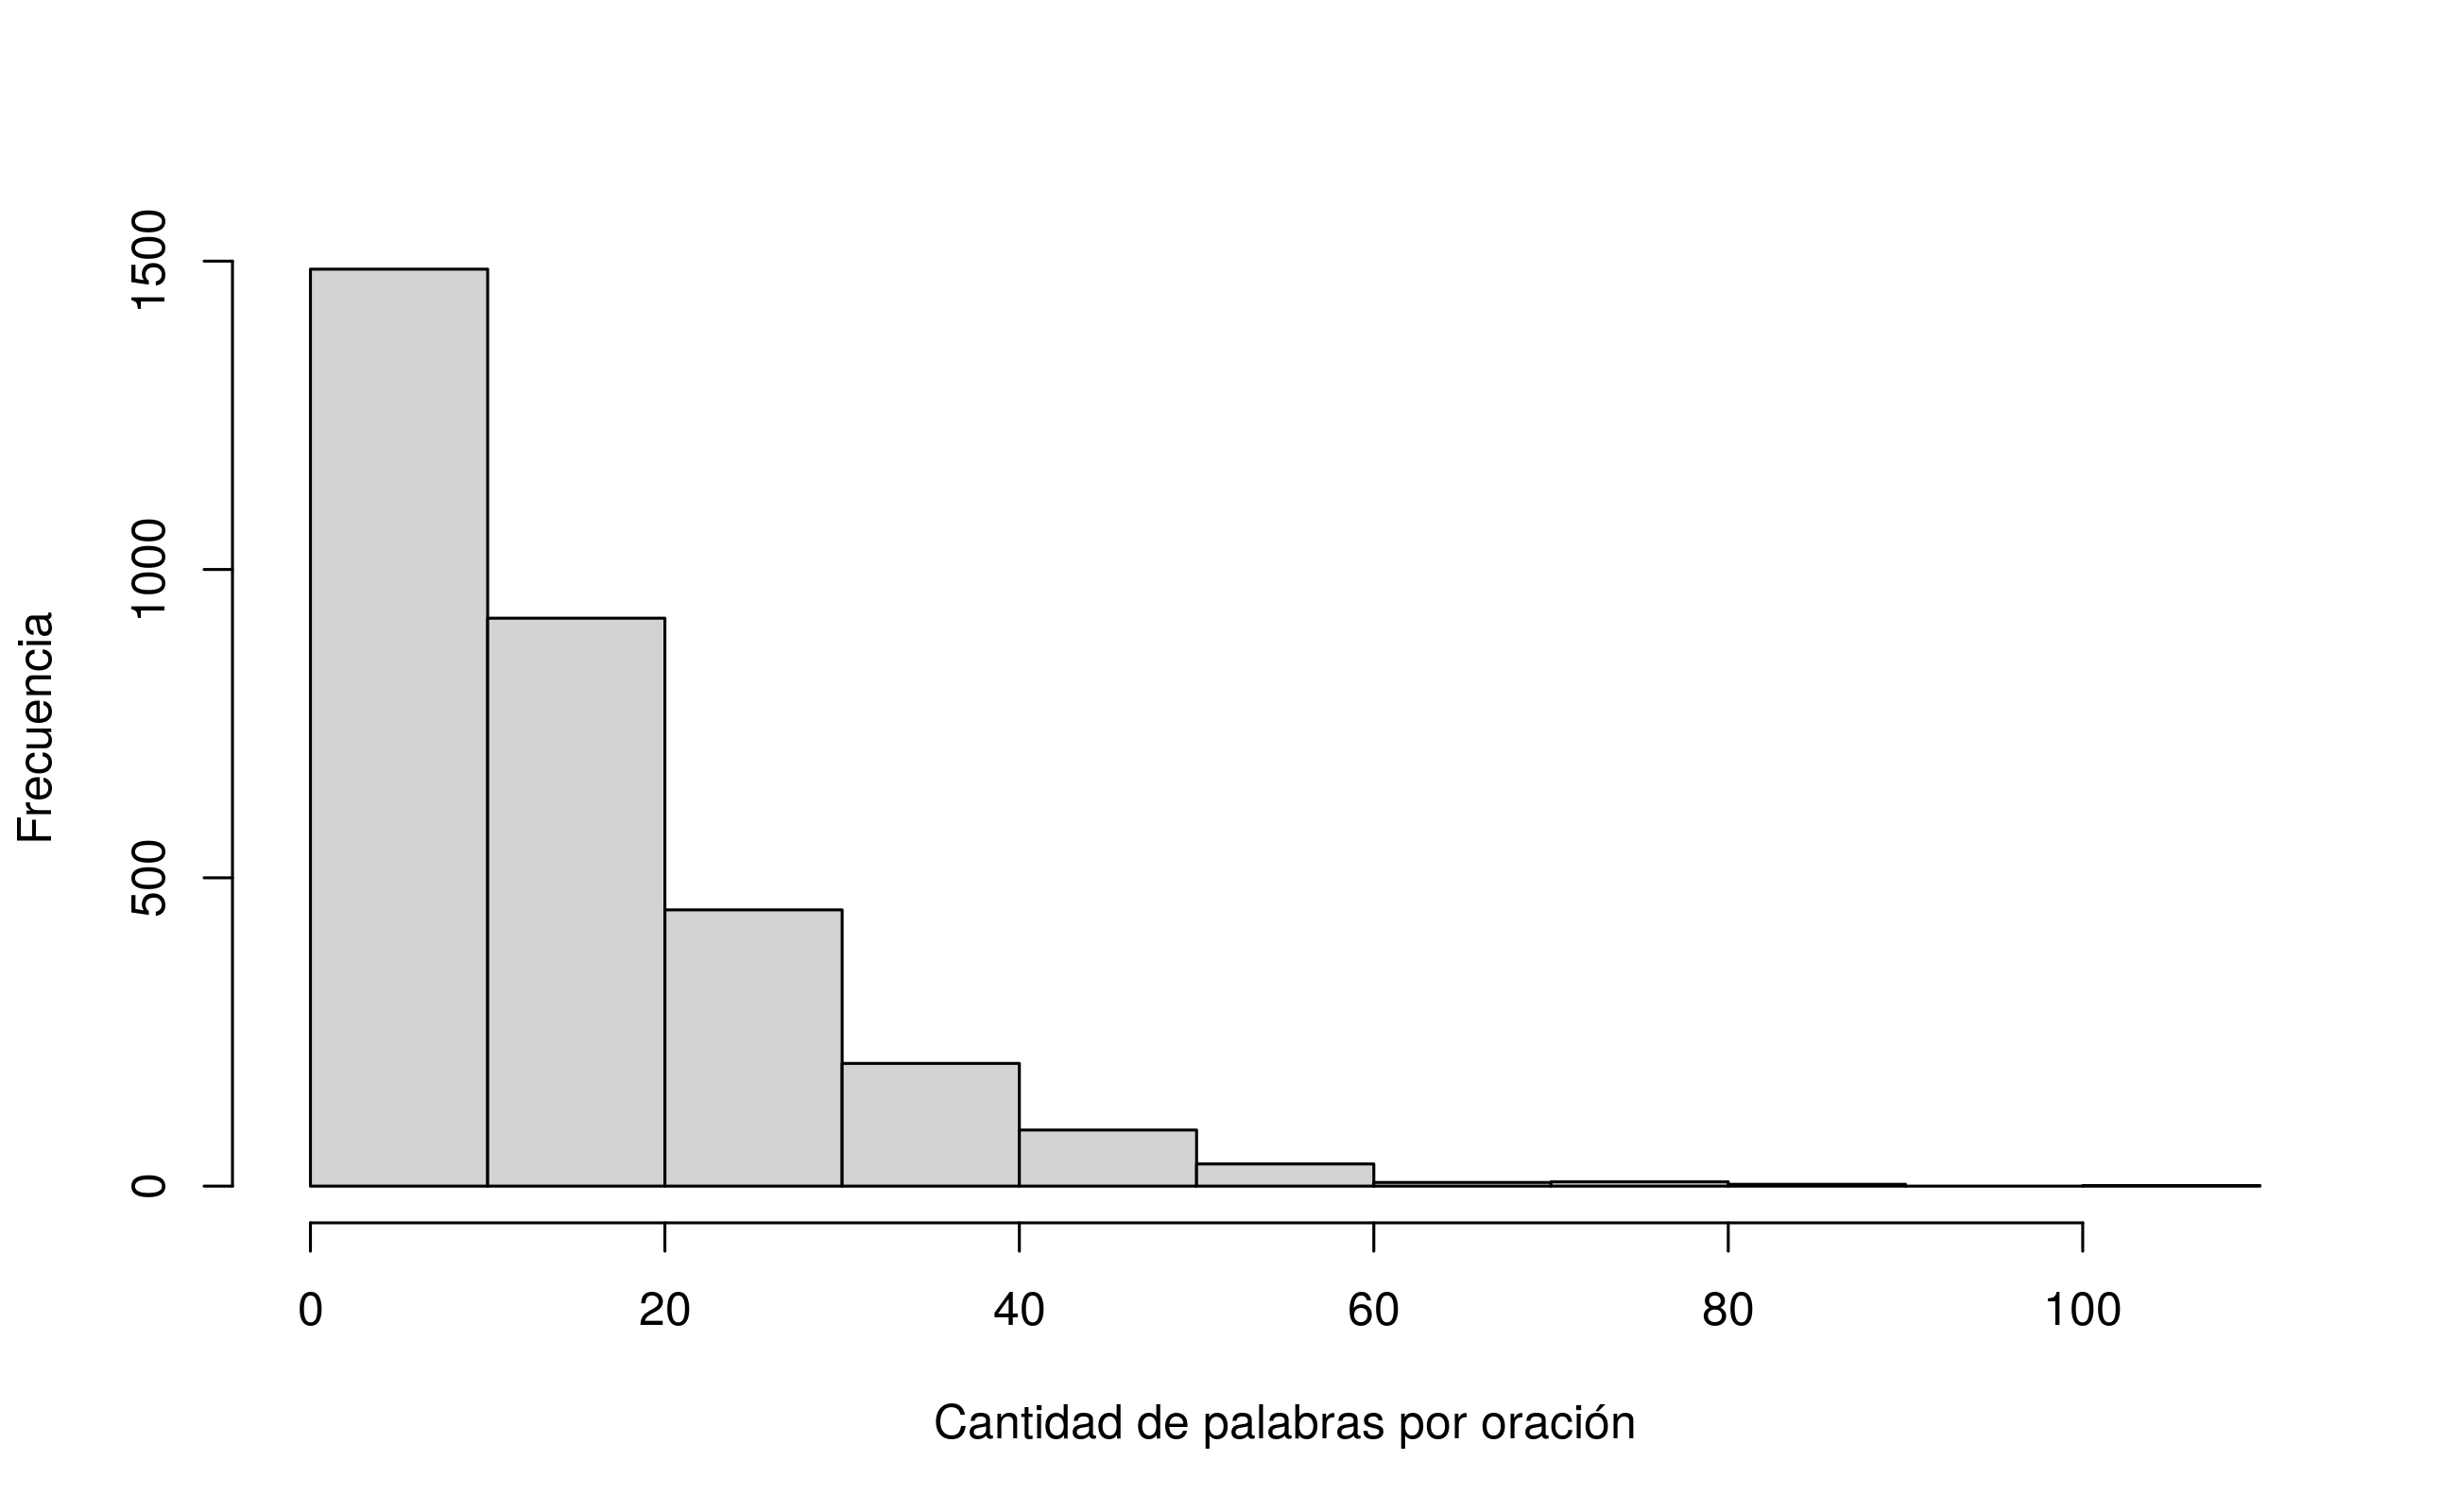
\includegraphics[scale=0.4]{hist_ppo_peter.png}
			\caption{Palabras por oración en \em Peter Pan}
			\label{ppo_peter}
		\end{subfigure}
				\begin{subfigure}{.5\textwidth}
			\centering
			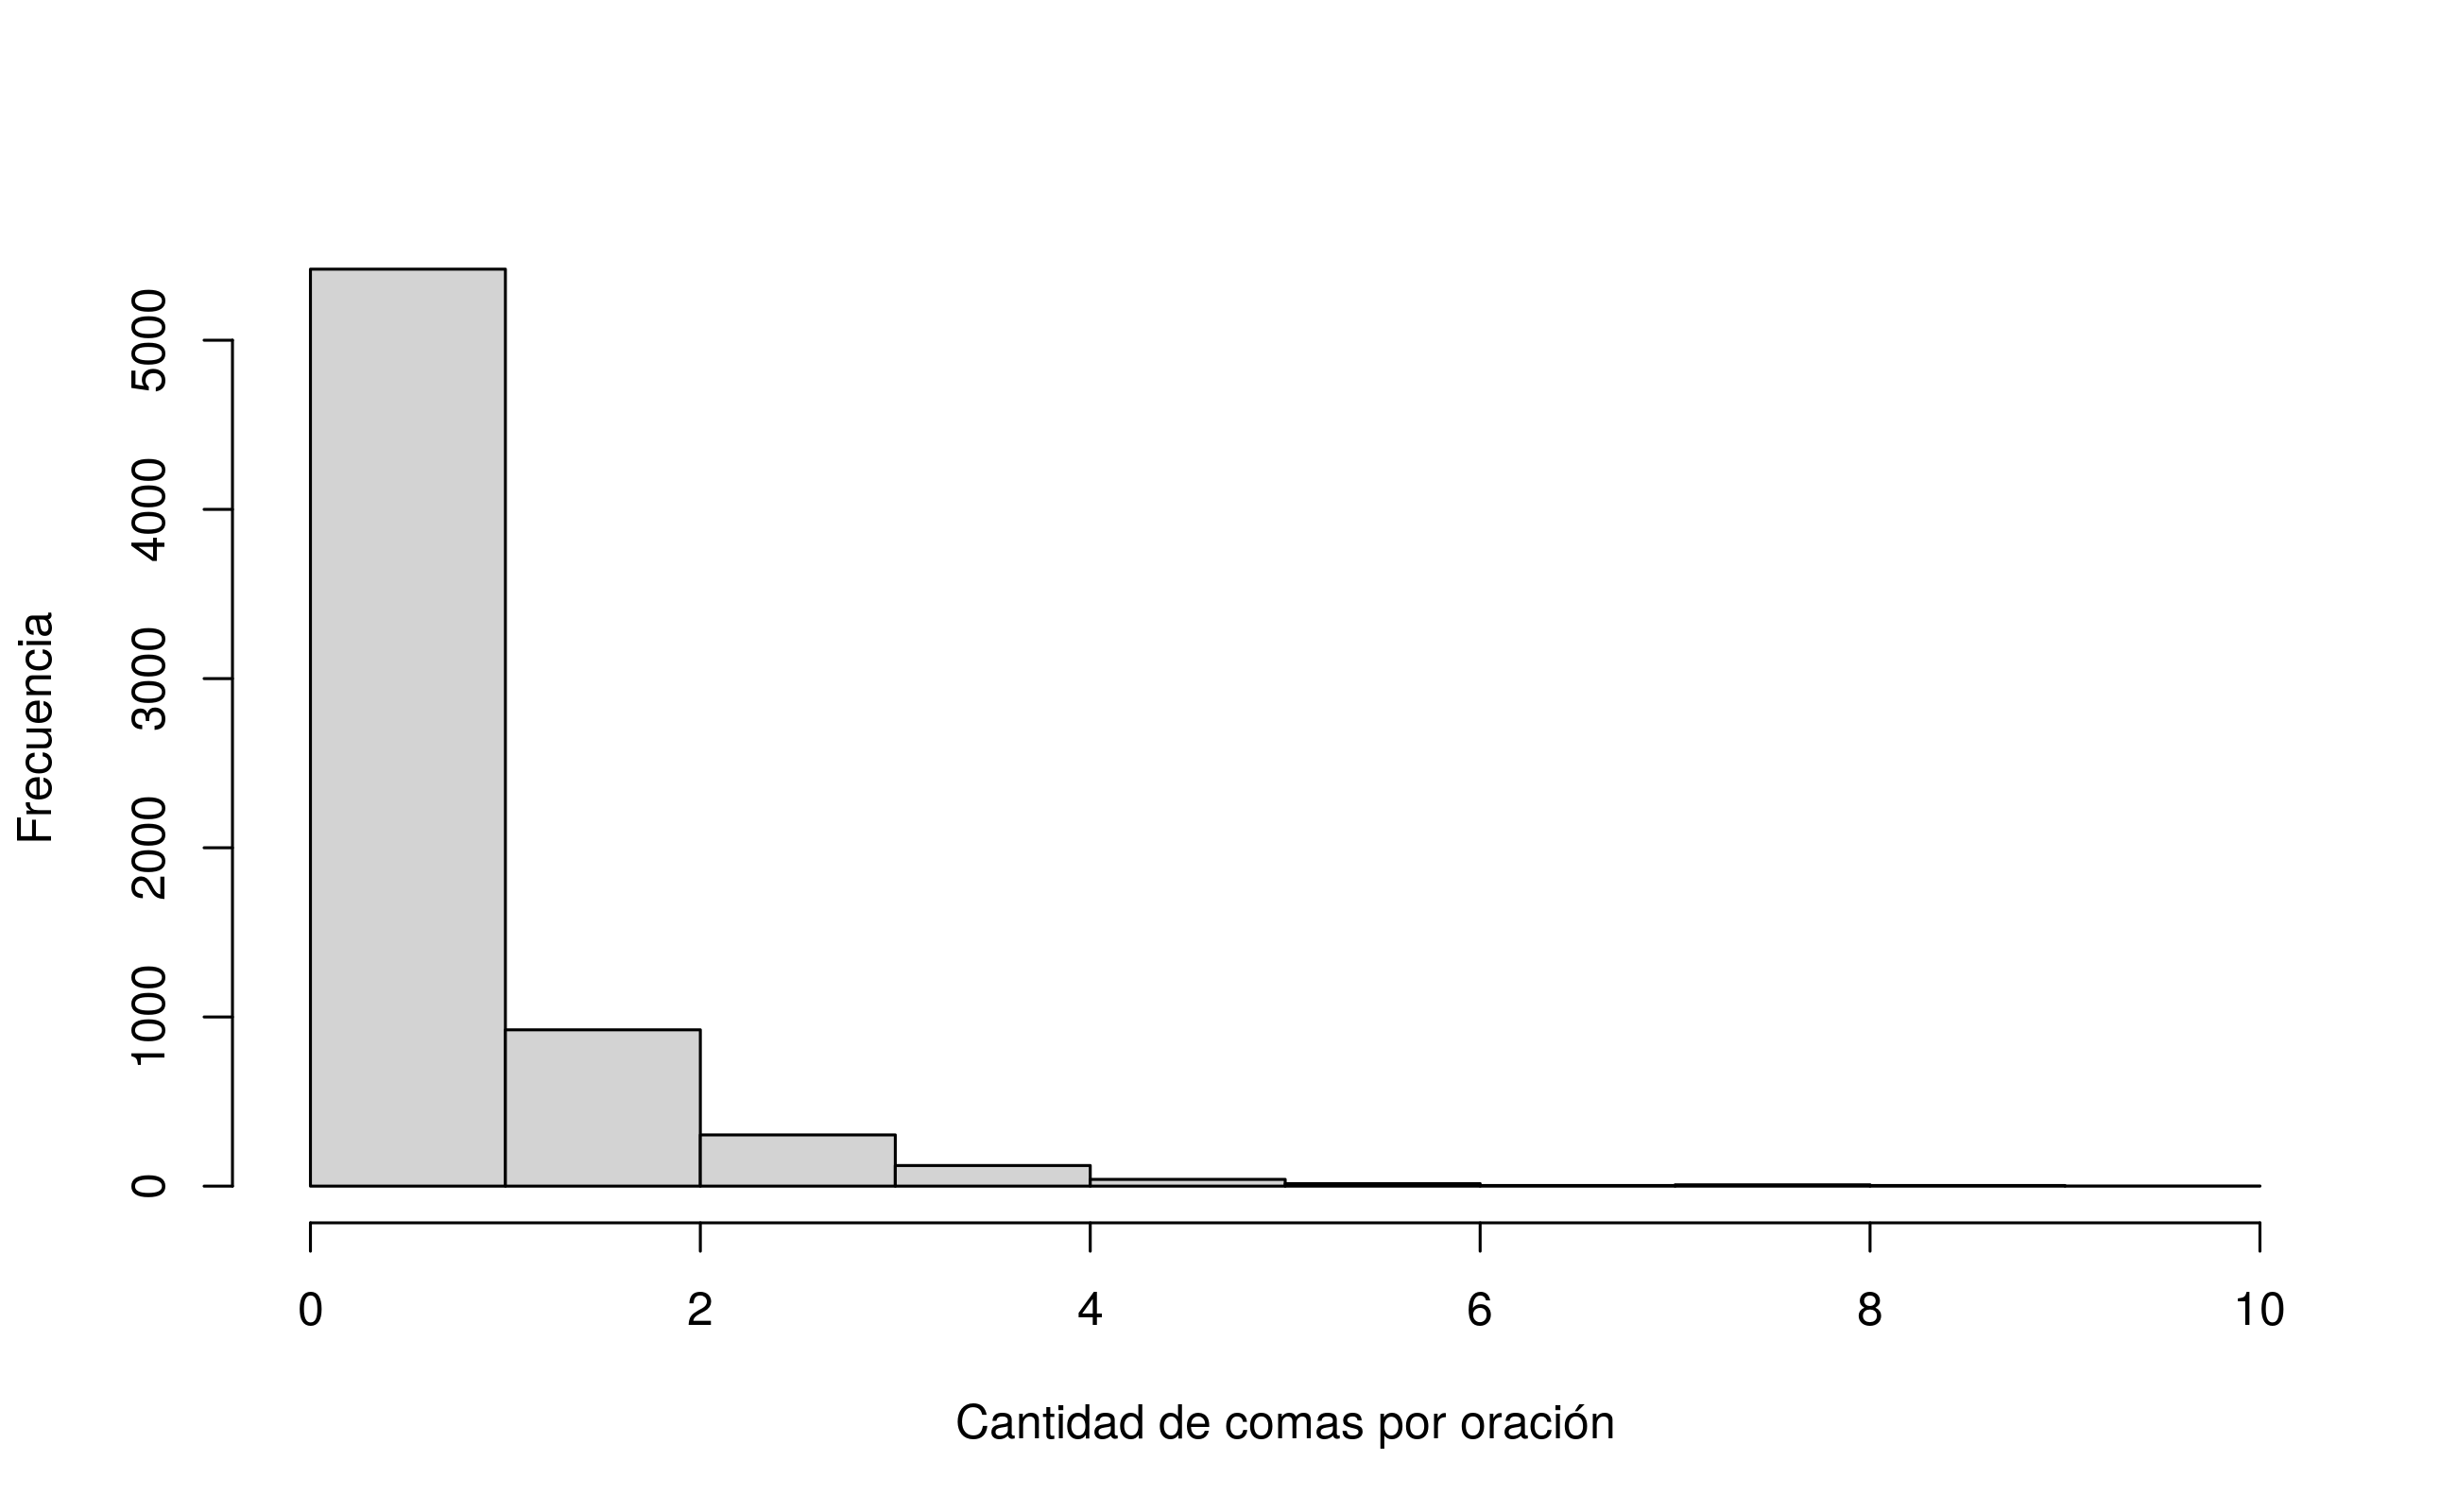
\includegraphics[scale=0.4]{hist_cpo_anne.png}
			\caption{Comas por oración en \em Anne of Green Gables}
			\label{cpo_anne}
		\end{subfigure}
		\begin{subfigure}{0.5\textwidth}
			\centering
			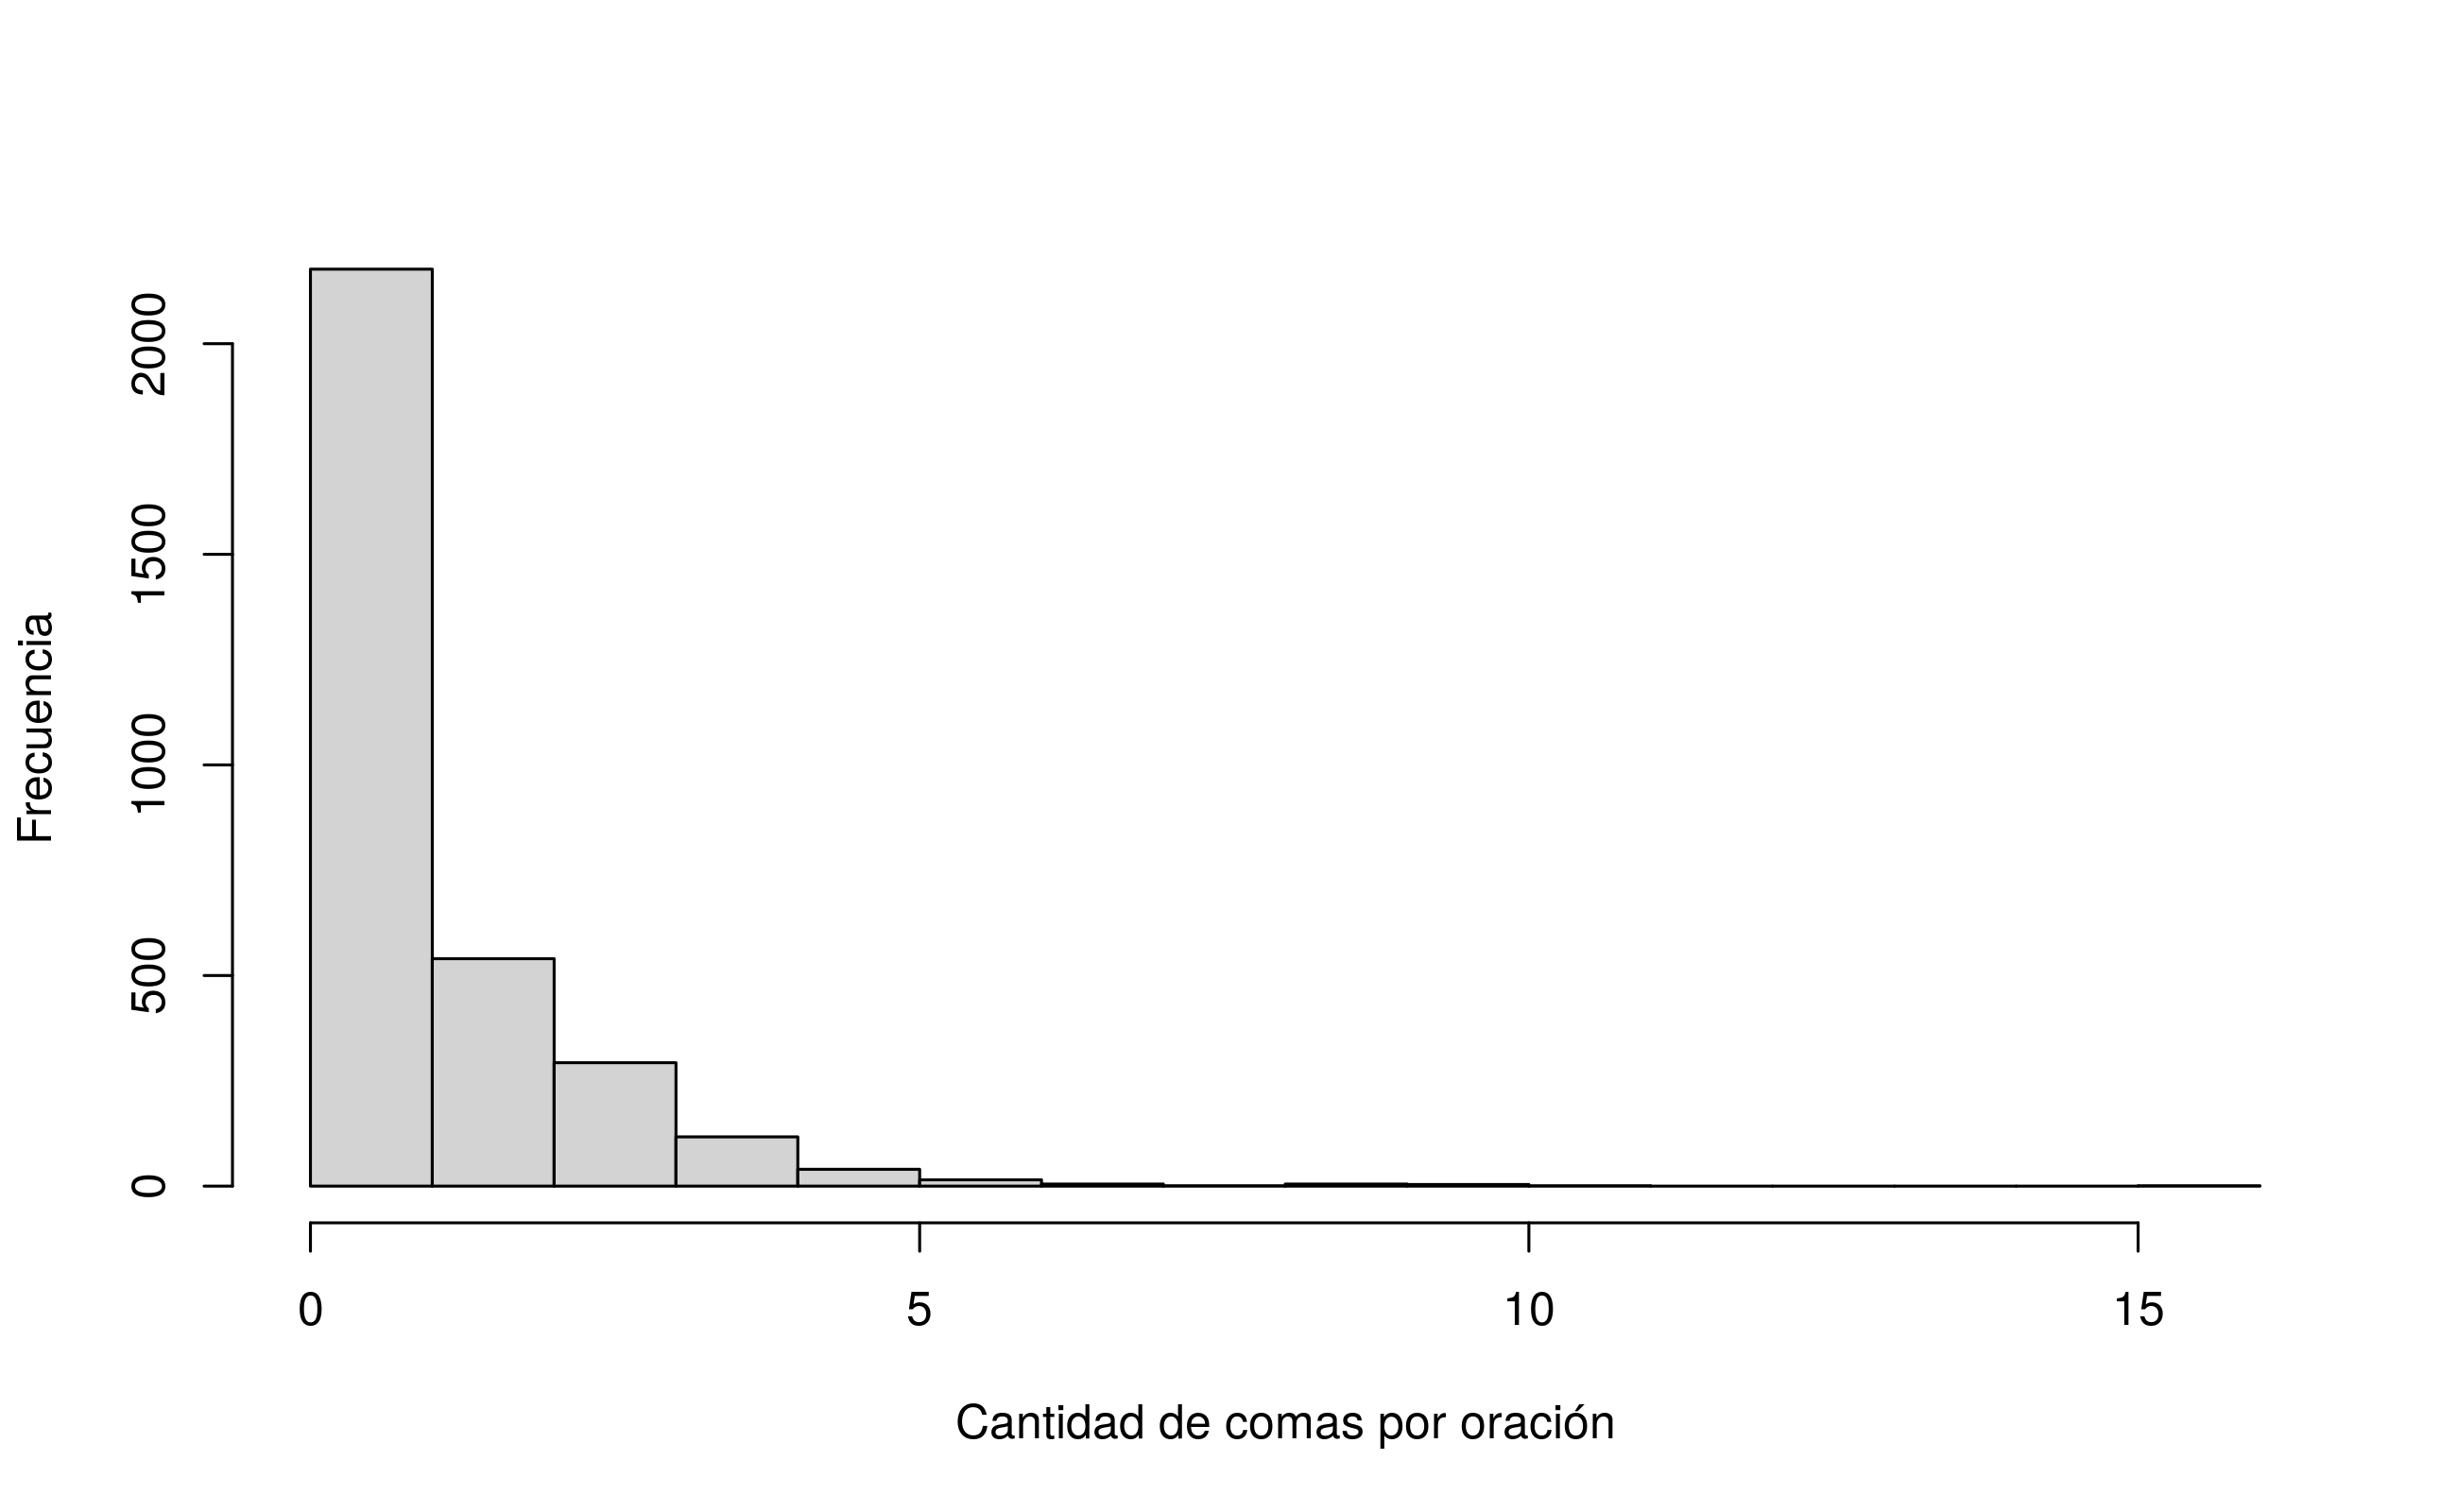
\includegraphics[scale=0.4]{hist_cpo_peter.png}
			\caption{Comas por oración en \em Peter Pan}
			\label{cpo_peter}
		\end{subfigure}
		\begin{subfigure}{.5\textwidth}
			\centering
			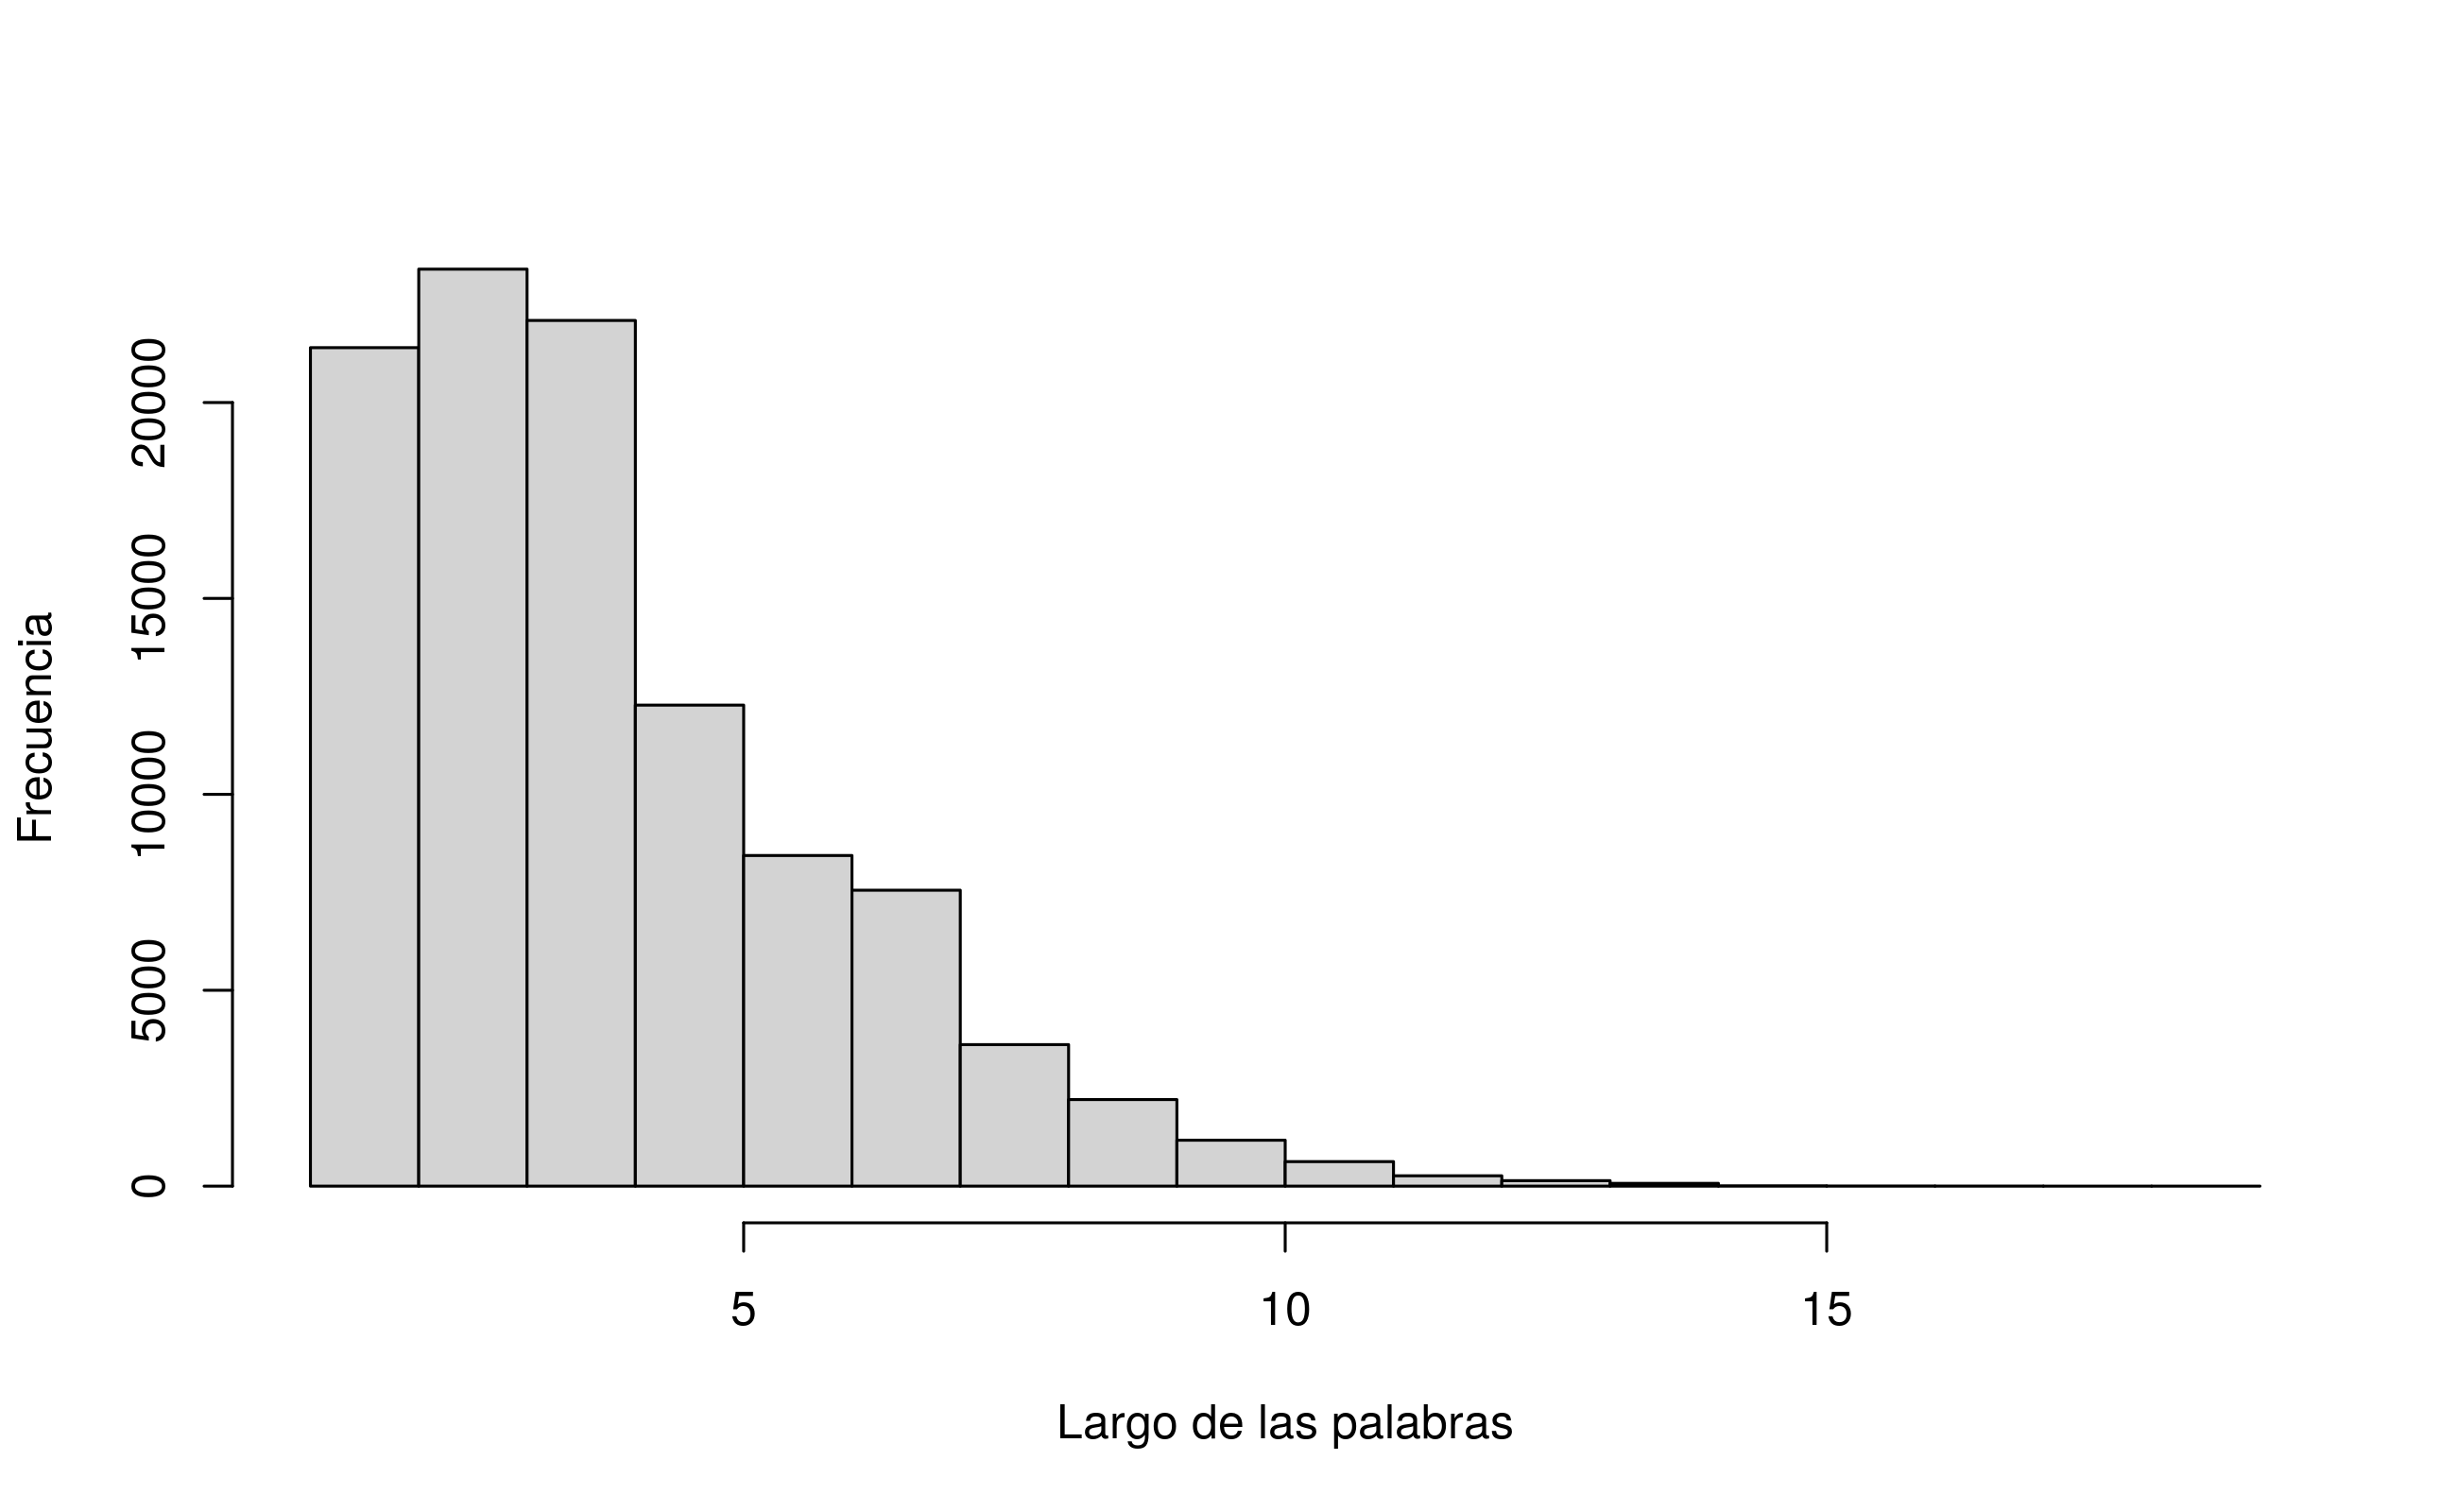
\includegraphics[scale=0.4]{hist_tpalabras_anne.png}
			\caption{Largo de palabras en \em Anne of Green Gables}
			\label{tpalabras_anne}
		\end{subfigure}
		\begin{subfigure}{0.5\textwidth}
			\centering
			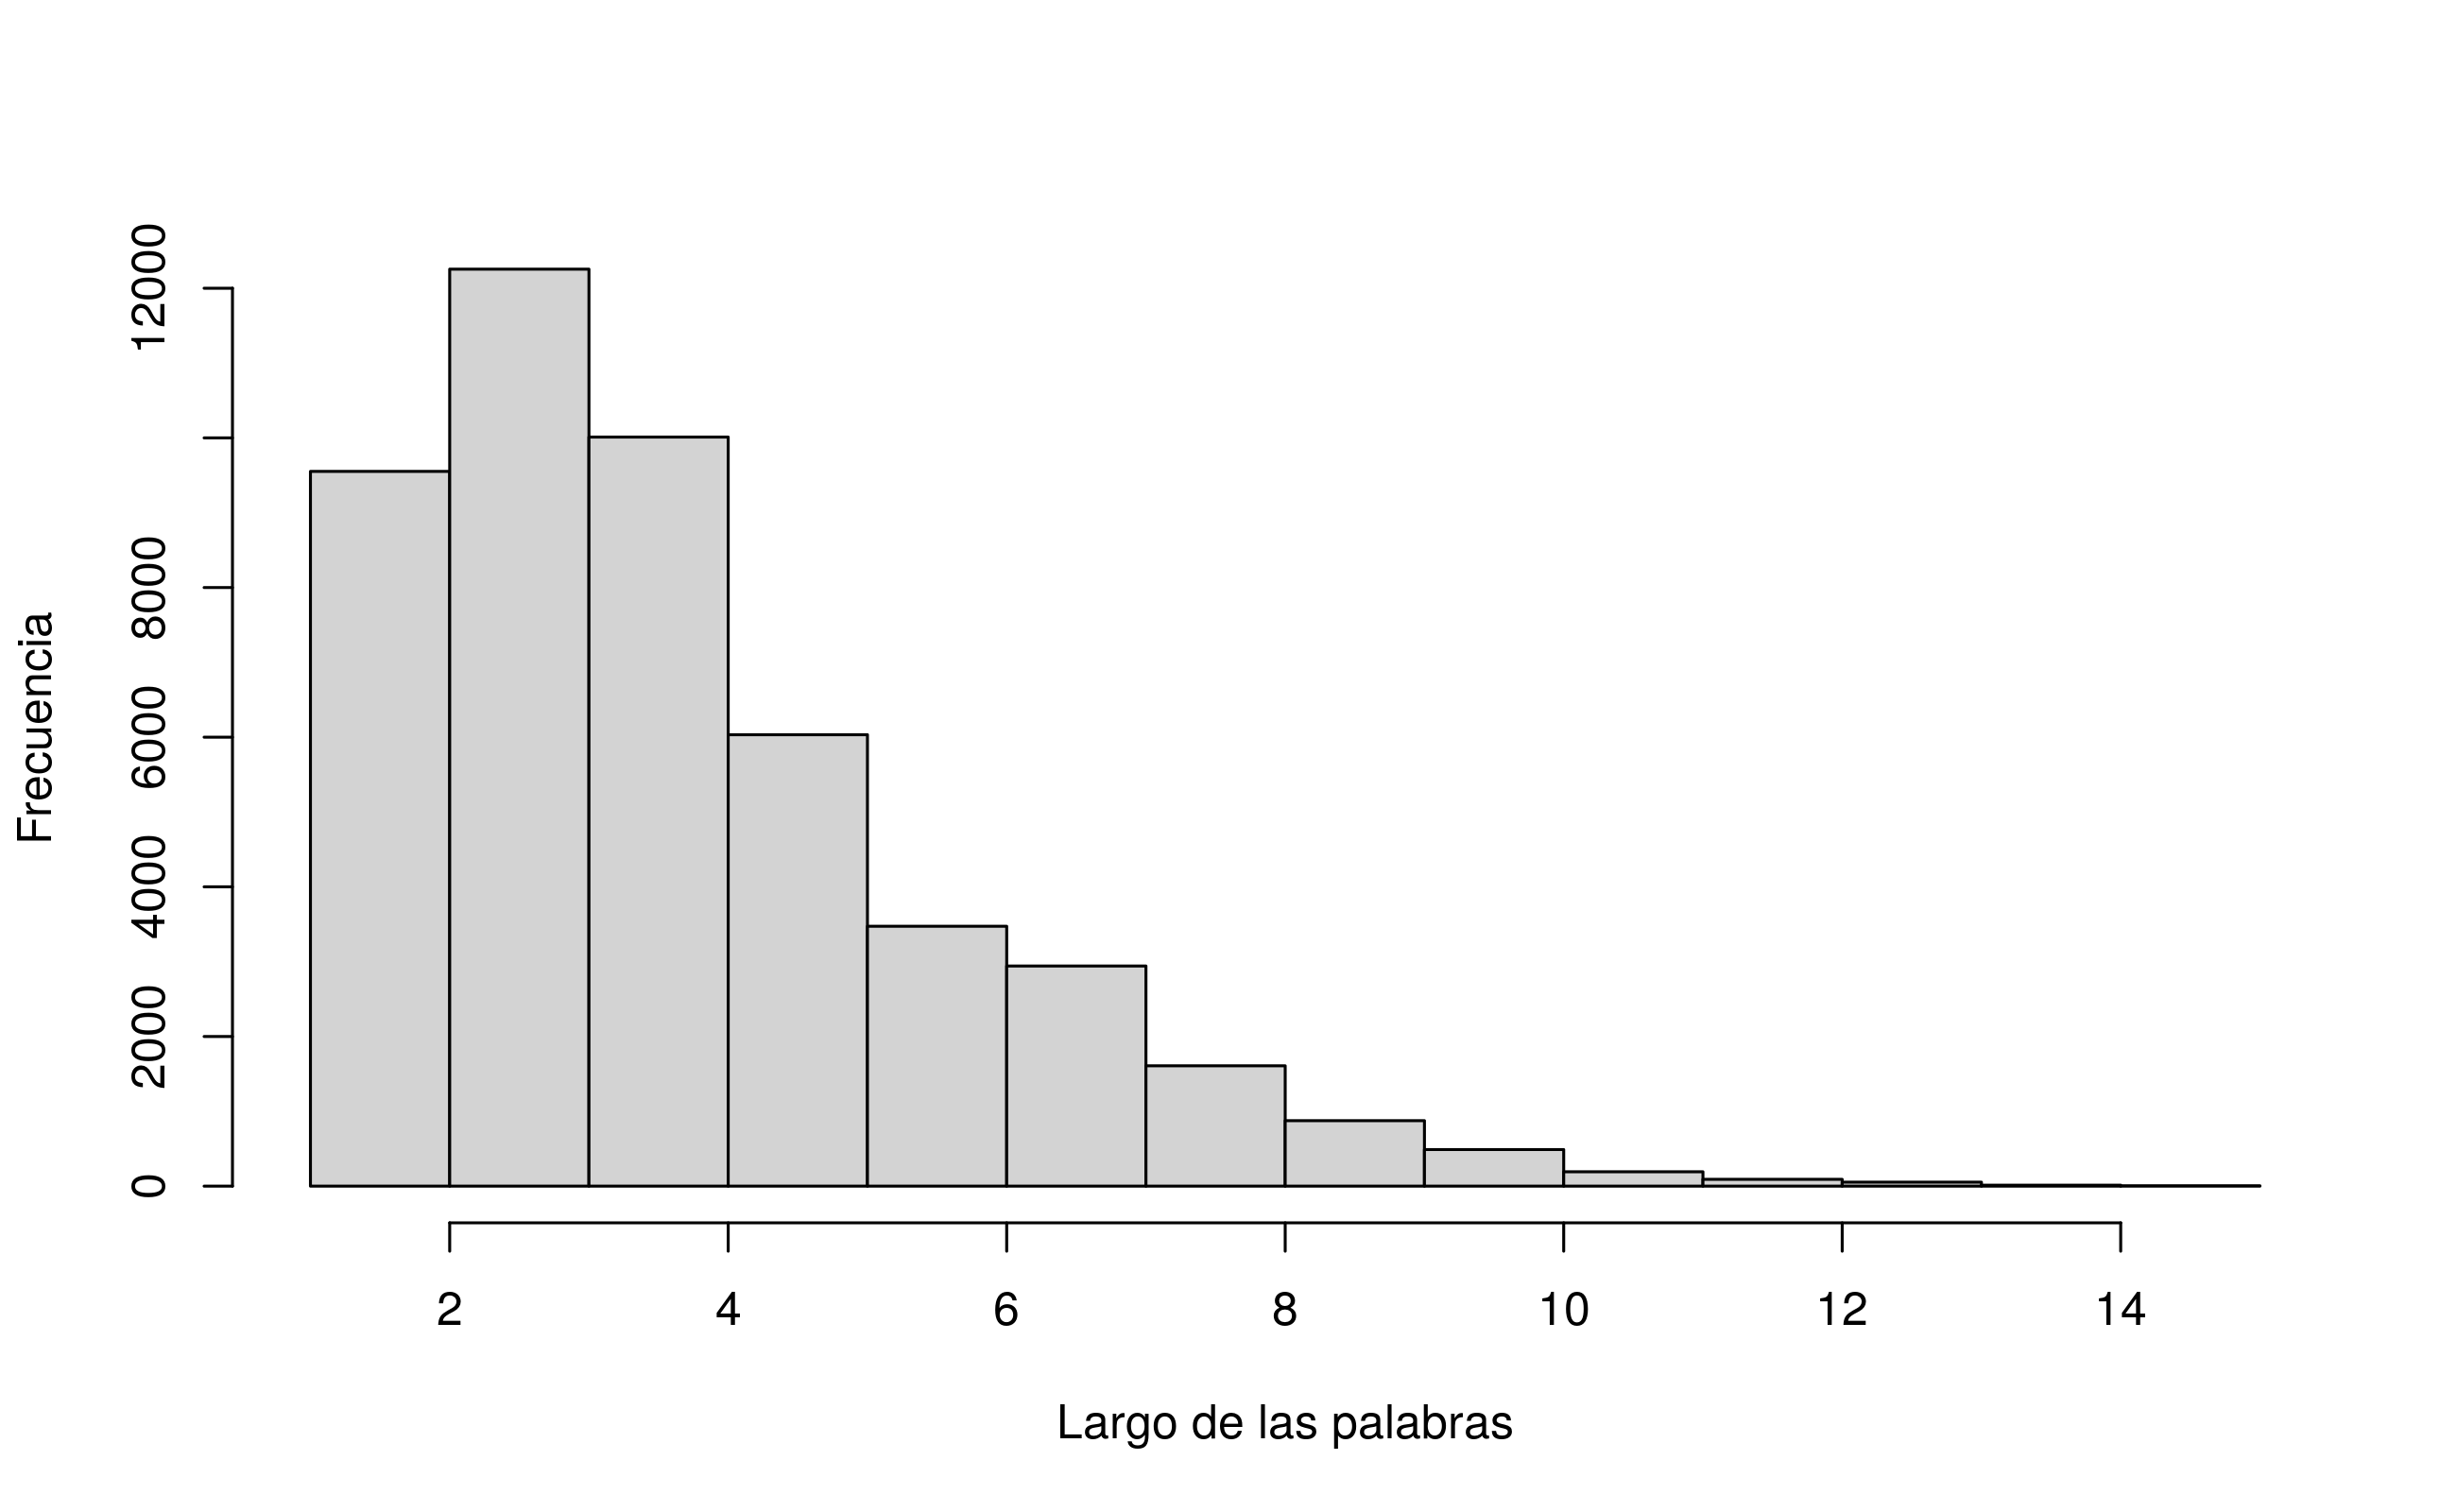
\includegraphics[scale=0.4]{hist_tpalabras_peter.png}
			\caption{Largo de palabras en \em Peter Pan}
			\label{tpalabras_peter}
		\end{subfigure}
		\caption{Síntesis de la distribución de las oraciones en los textos.}
		\label{anne_peter}
	\end{figure}

 
	
	\subsection{Experimentos de Bernoulli}
	
	Para esta fase se usa solo el texto de {\em Anne of Green Gables}. A partir de esa información se realizan distintos experimentos de Bernoulli que buscan imitar el comportamiento de tres distribuciones: geométrica, binomial y binomial negativa.
	
	La distribución geométrica muestra la distribución de la cantidad de repeticiones del experimento que fueron fracasos antes de obtener el primer éxito \cite{notas_mpa}. Para replicar este comportamiento se define que el éxito se obtiene cuando al elegir al azar una letra del texto esta es una ``e'', por lo tanto, si se obtiene cualquier otro caracter se considera un fracaso. Al repetir 10,000 veces el experimento se obtienen los resultados de la figura \ref{geom_e}. Por la construcción del experimento, es claro que el comportamiento sigue una distribución geométrica.
	
	\begin{figure}
		\centering
		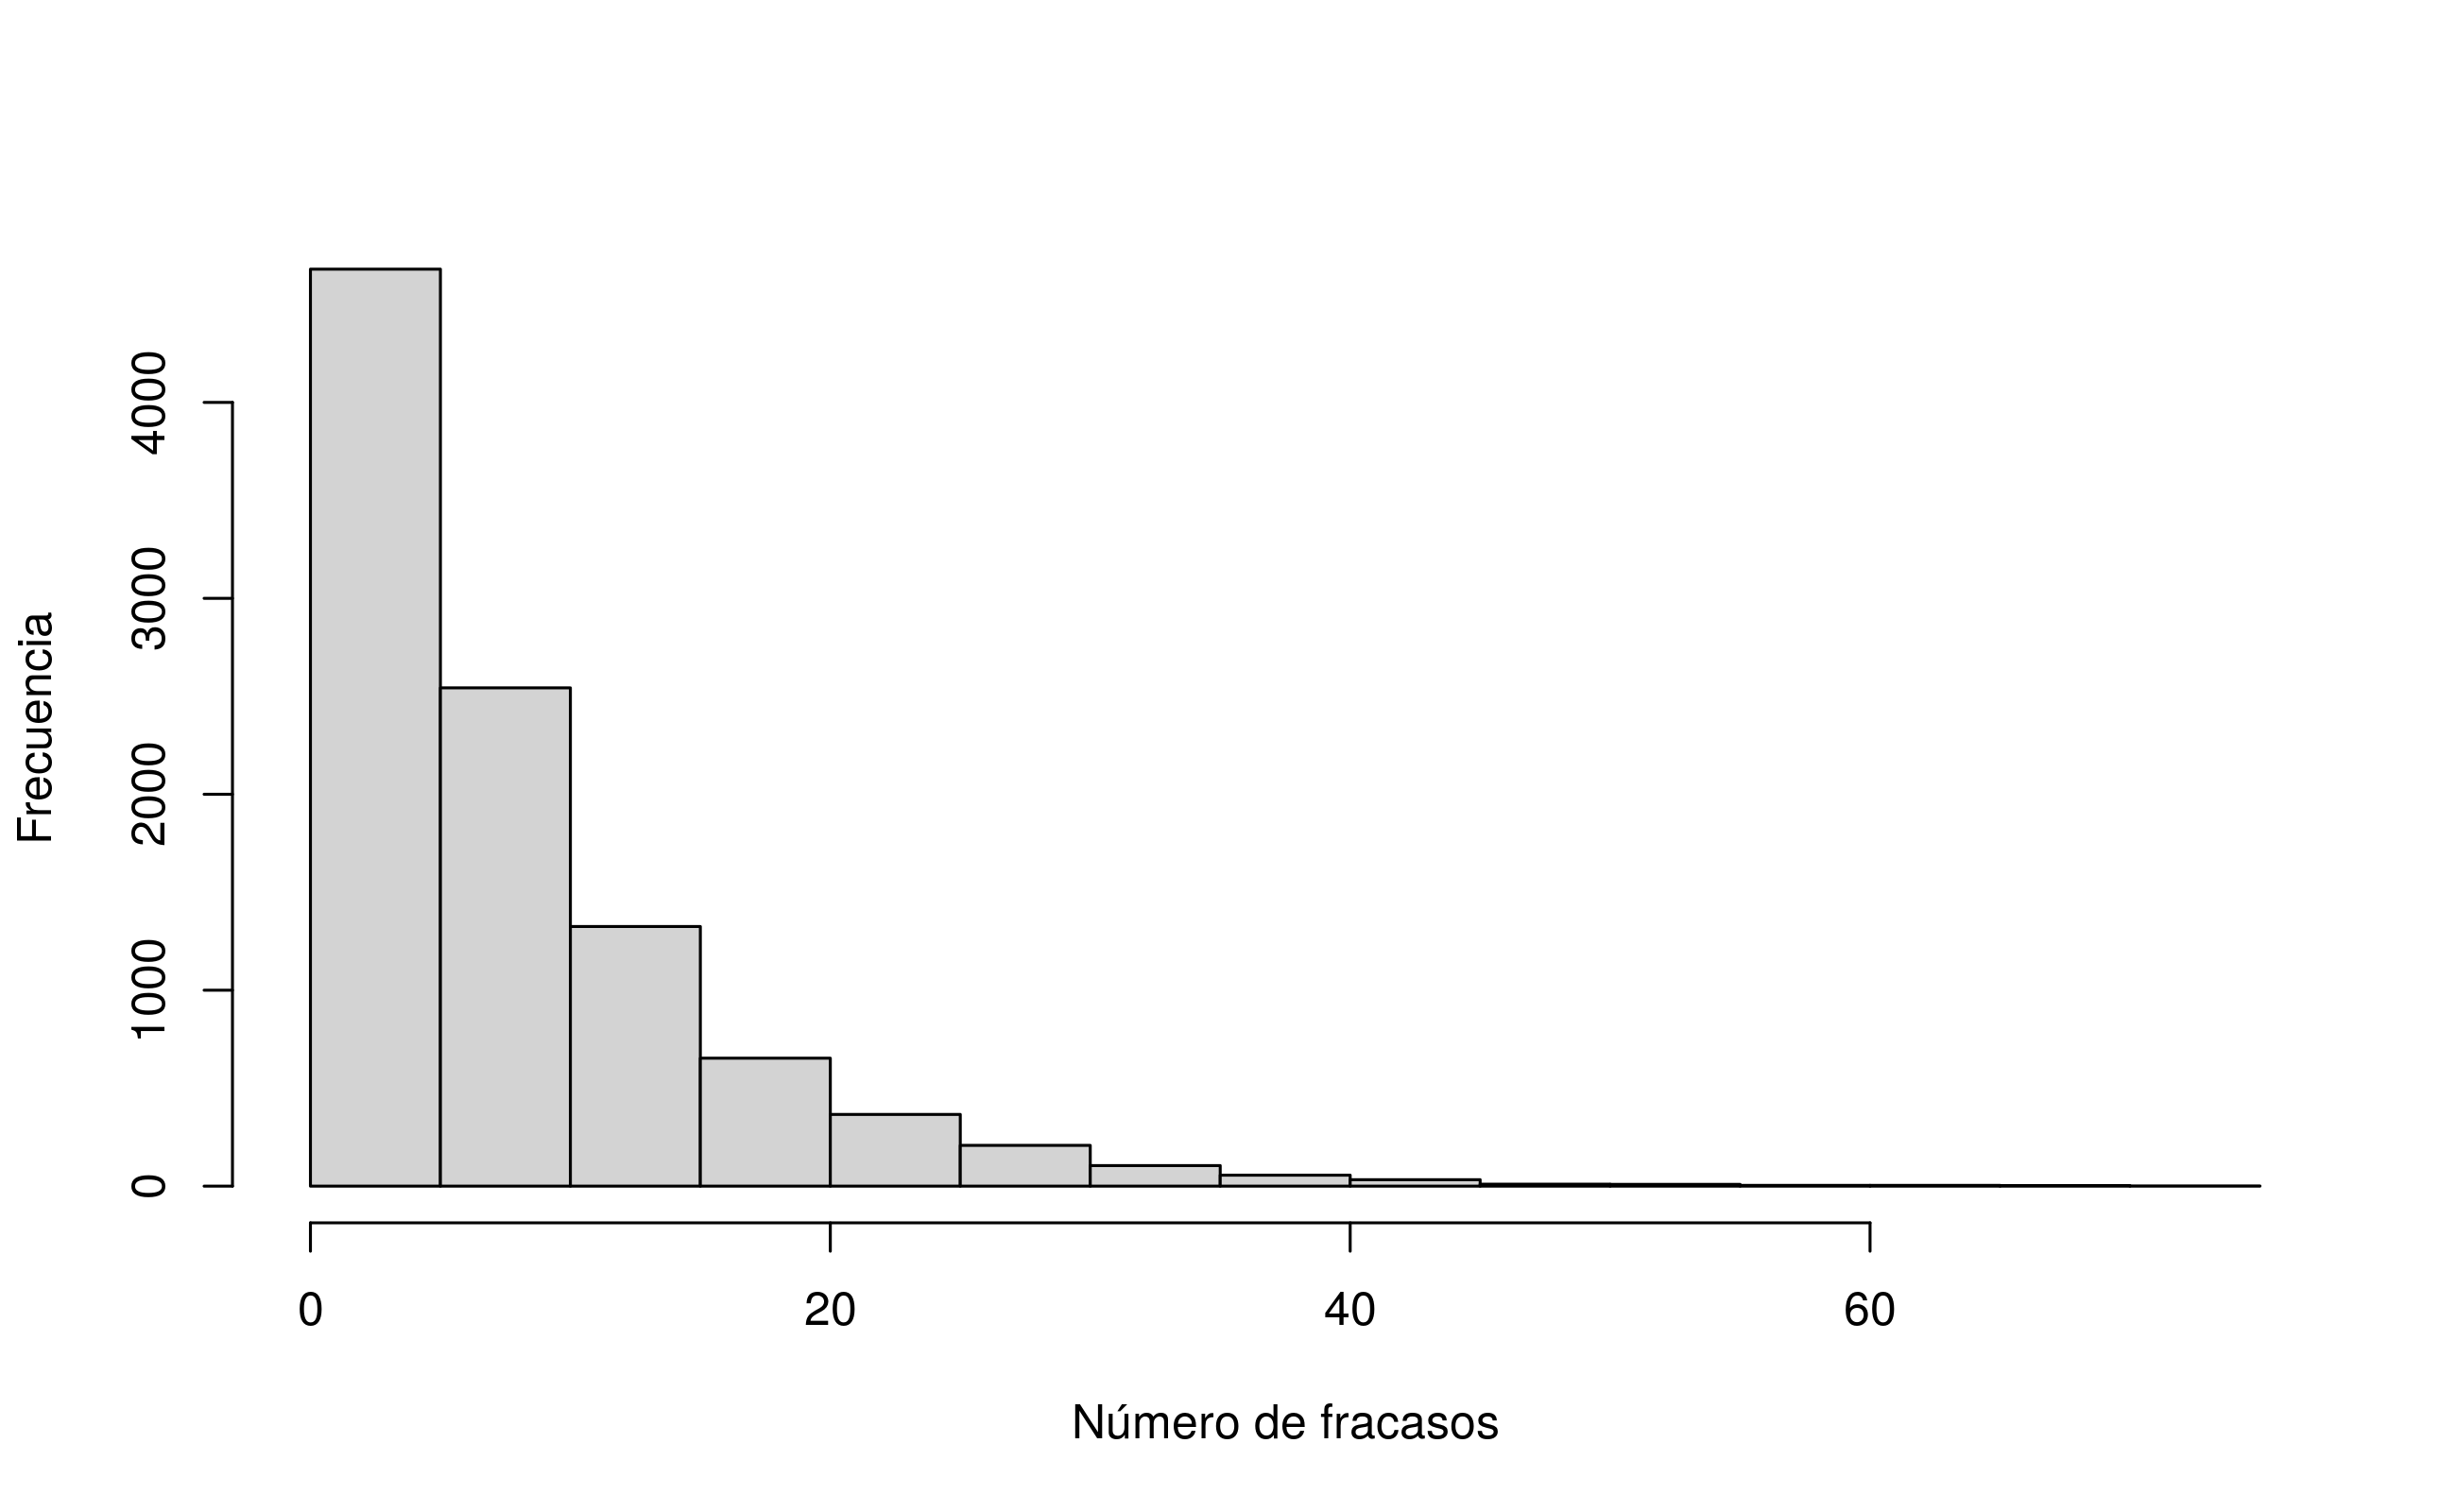
\includegraphics[scale=0.6]{geom_e.png}
		\caption{Distribución geométrica.}
		\label{geom_e}
	\end{figure}

	El siguiente experimento contesta a la pregunta ¿cuántos intentos se necesitan para obtener siete veces el caracter ``t'', en una elección al azar?. Un éxito, para este experimento, se considera cuando en la elección se obtiene el caracter ``t''. Esta distribución se conoce como binomial negativa. En la figura \ref{bin_neg_t7} se muestran los resultados obtenidos al repetir 10,000 veces el experimento.
	
	\begin{figure}
		\centering
		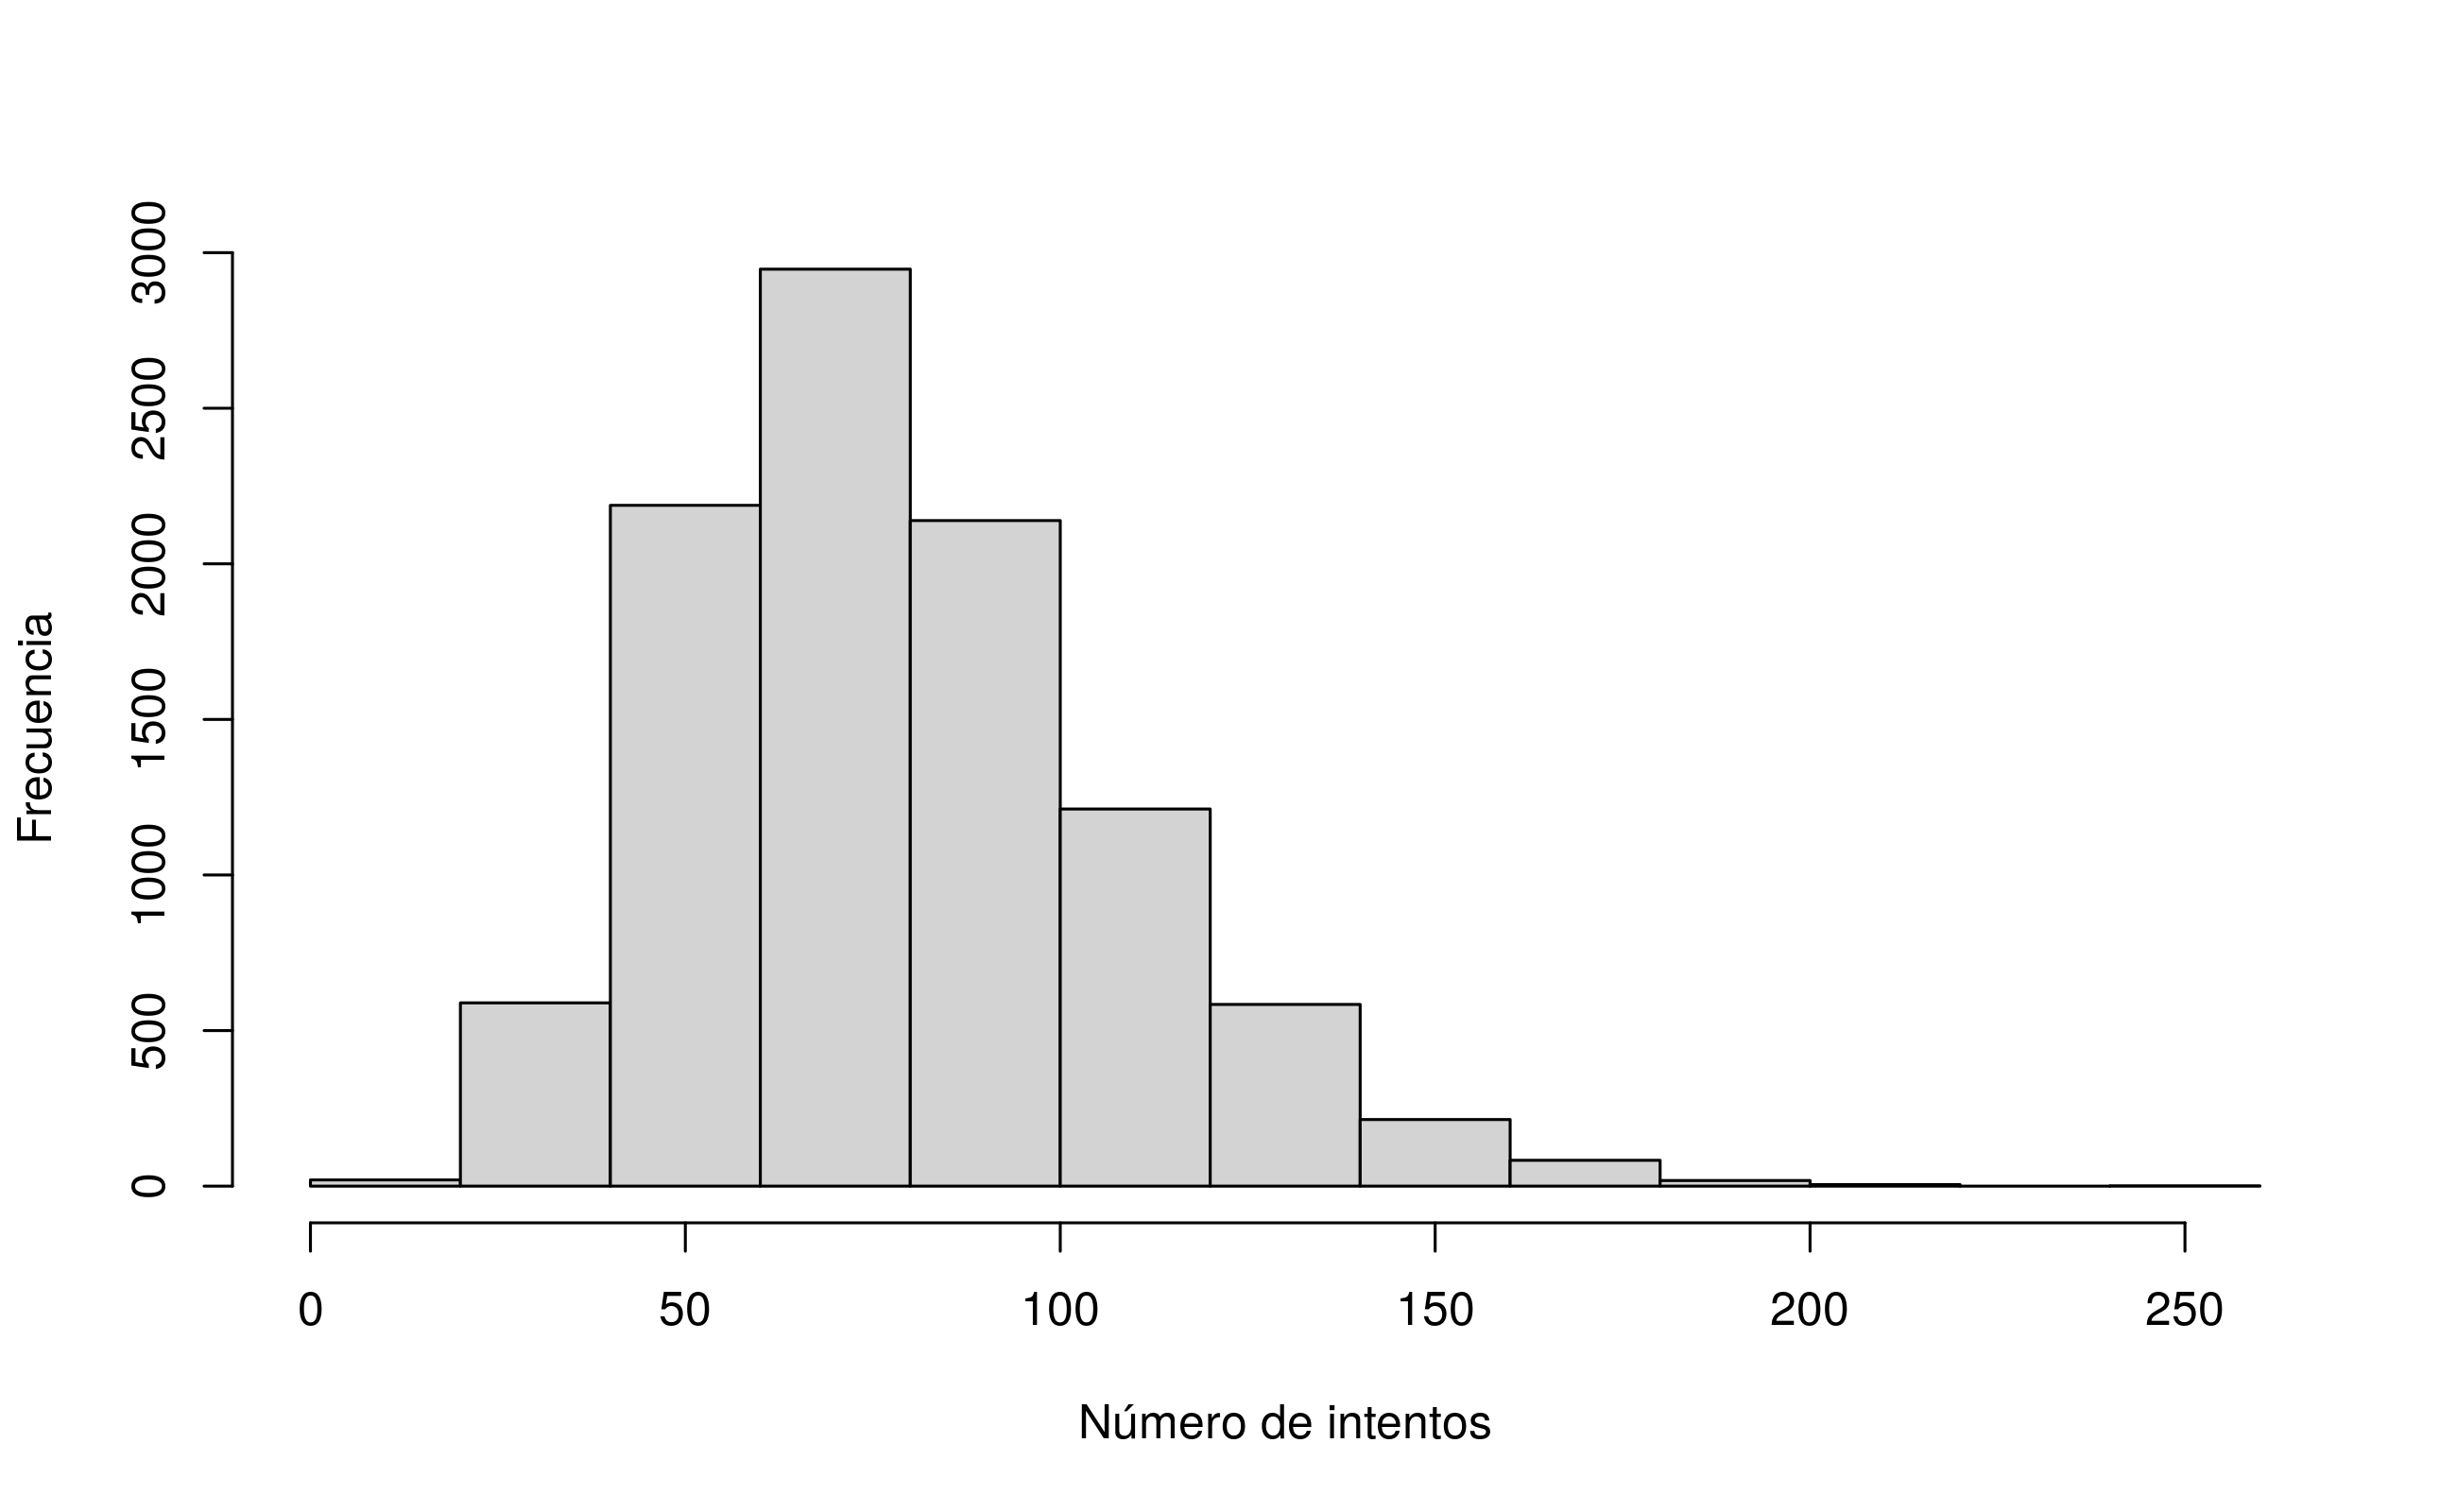
\includegraphics[scale=0.6]{bin_neg_t7.png}
		\caption{Distribución binomial negativa.}
		\label{bin_neg_t7}
	\end{figure}
	
	La última situación considera un experimento de 30 intentos que se replica 1,000 veces. En cada réplica se cuenta la cantidad de veces que se elige al azar una palabra y ésta tiene una longitud menor o igual a cinco caracteres. La distribución obtenida de este experimento se muestra en la figura \ref{bin_5}. La construcción del experimento permite concluir que este comportamiento es el de una distribución binomial.
	
	La distribución en la figura \ref{tpalabras_anne} indica que la mayoría de las palabras en el texto tiene una longitud menor o igual a cinco caracteres. De esta forma en el experimento de elegir 30 palabras al azar, se espera que la mayoría de ellas tenga esta restricción en la longitud es por esto que se observa el comportamiento de la figura \ref{bin_5}. 
	
	\begin{figure}
		\centering
		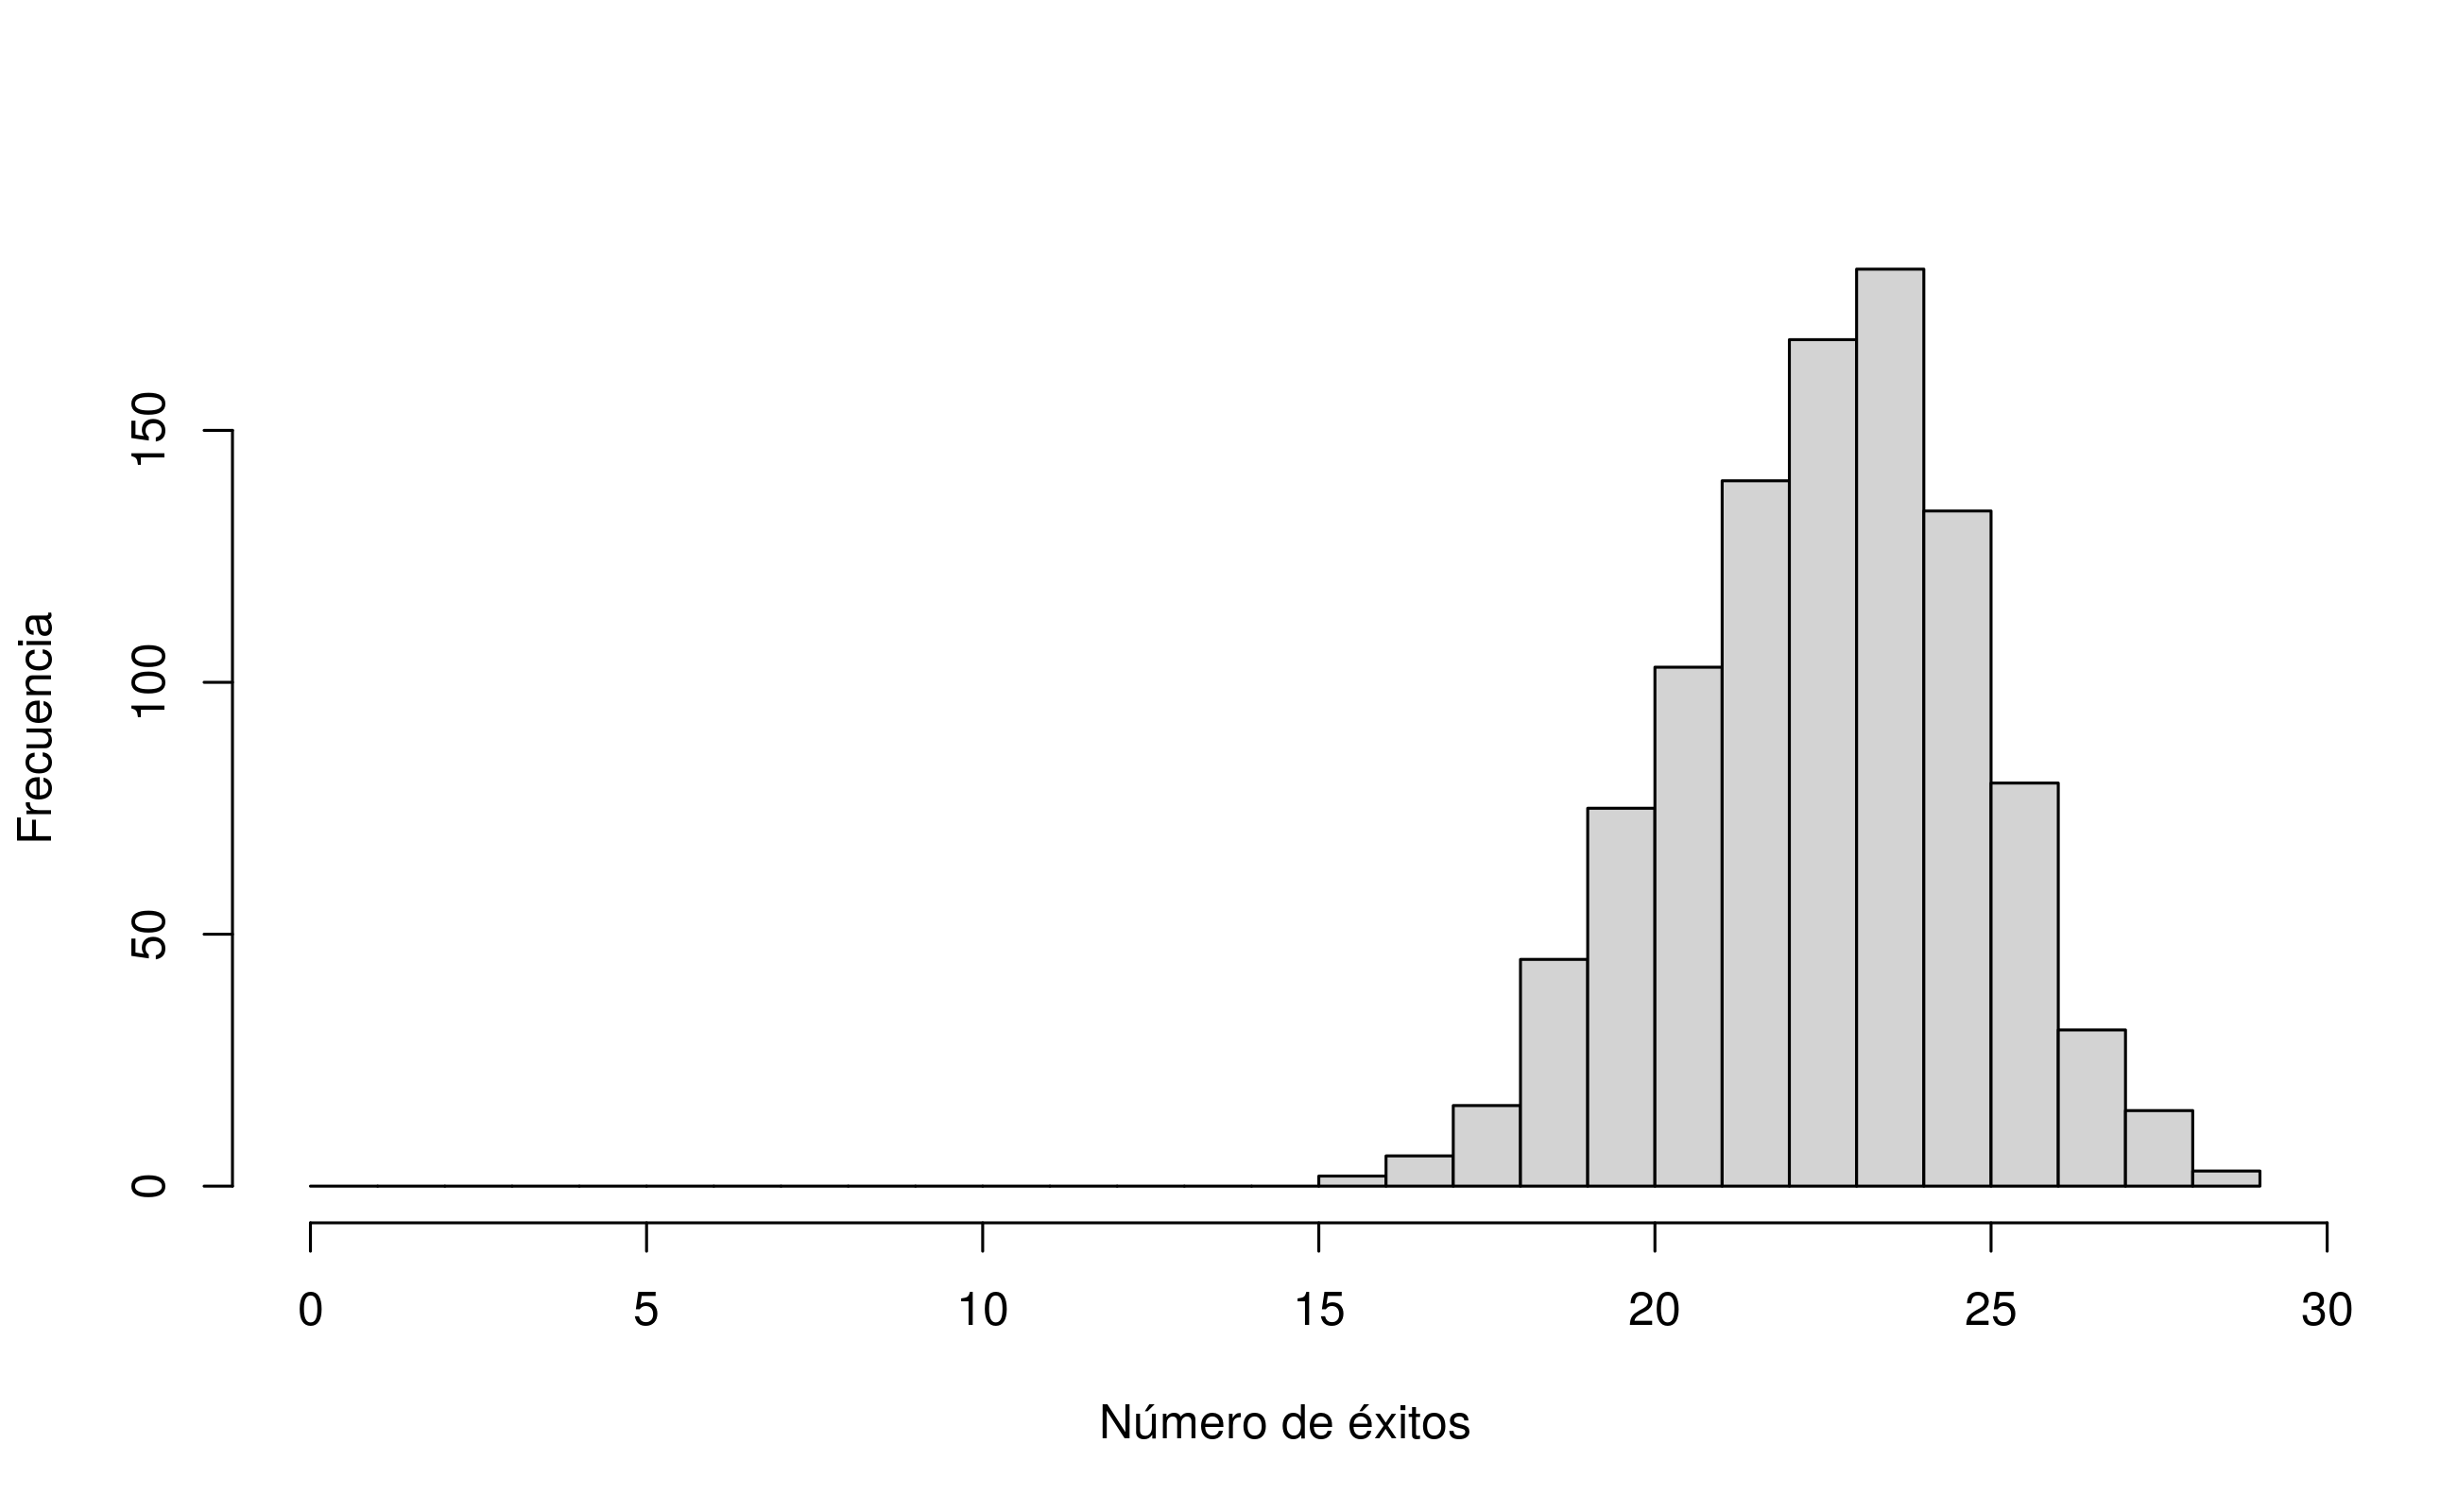
\includegraphics[scale=0.6]{bin_5.png}
		\caption{Distribución binomial.}
		\label{bin_5}
	\end{figure}
	
\bibliographystyle{plain}
\bibliography{biblio}



\end{document}

